%pb
\documentclass[../../main/main.tex]{subfiles}

\pagenumbering{arabic}
\begin{document}


%%%%%%%%%%%%%%%%%%%%% Chapter Patrol Base Operations %%%%%%%%%%%%%%%
\chapter{Patrol Base Operations}
This is the future works section. But, as I am typing this, it is the current working section for \LaTeX\.  The point here is to get the margins in order.   This means that there must be text of sufficient length to visually verify that the text meets LORI's standards.  LORI is complying with SU standards for the senior thesis.  Therefore, meeting LORI's standards is synonymous with meeting SU's standards.  Resistance will only degrade you.
   %%%%%%%%%%%%%%%%%%%% Section Motivation %%%%%%%%%%%%%%%%%%%%%%
\section{Motivation}
The patrol base operations described in the patrol base Ranger Handbook

   %%%%%%%%%%%%%%%%%%% Section Ranger Handbook Description %%%%%%%%%%%%%
\section{Ranger Handbook Description}

   %%%%%%%%%%%%%%%%%%% Section Describing The Patrol Base Operations %%%%%%%%
\section{Modeling the Patrol Base Operations from the Ranger Handbook}\label{sec:modelingpb}
\glsresetall[\acronymtype]
Modeling a system requires the knowledge of an expert on the system.  This is necessary because only someone who is familiar with the system, especially with regards to security, can detail its nuances.  For this reason, a subject matter expert from the United States Army (Jesse Nathanial Hall) is employed to develop a model of the patrol base operations. 

The model of the patrol base operations needs to be amiable to complete mediation and verification using an access-control logic (section \ref{sec:acl}).  This is necessary to prove security properties of the patrol base operations.  To do this, the patrol base operations are abstracted from the Ranger Manual and modeled in Visio\footnote{This work began as a collaboration between Jesse and the author.  Once the hierarchy of secure state machines was decided upon, the abstraction of the Ranger Manual was done by Jesse Nathanial Hall with only structural consultation with the author.}  The result of doing this is a hierarchy of secure state machines (\glsentryshortpl{ssm}). (\glsentryshortpl{ssm} are described in section \ref{sec:ssm}.)  

Each level-of the hierarchy of \glsentryshortpl{ssm} represents a level of abstraction of the patrol base operations. The most abstract level of the hierarchy is the top level \glsentryshort{ssm}.  A diagram of this most abstract level is shown in figure \ref{pbtoplevel}.

\begin{figure}[h]
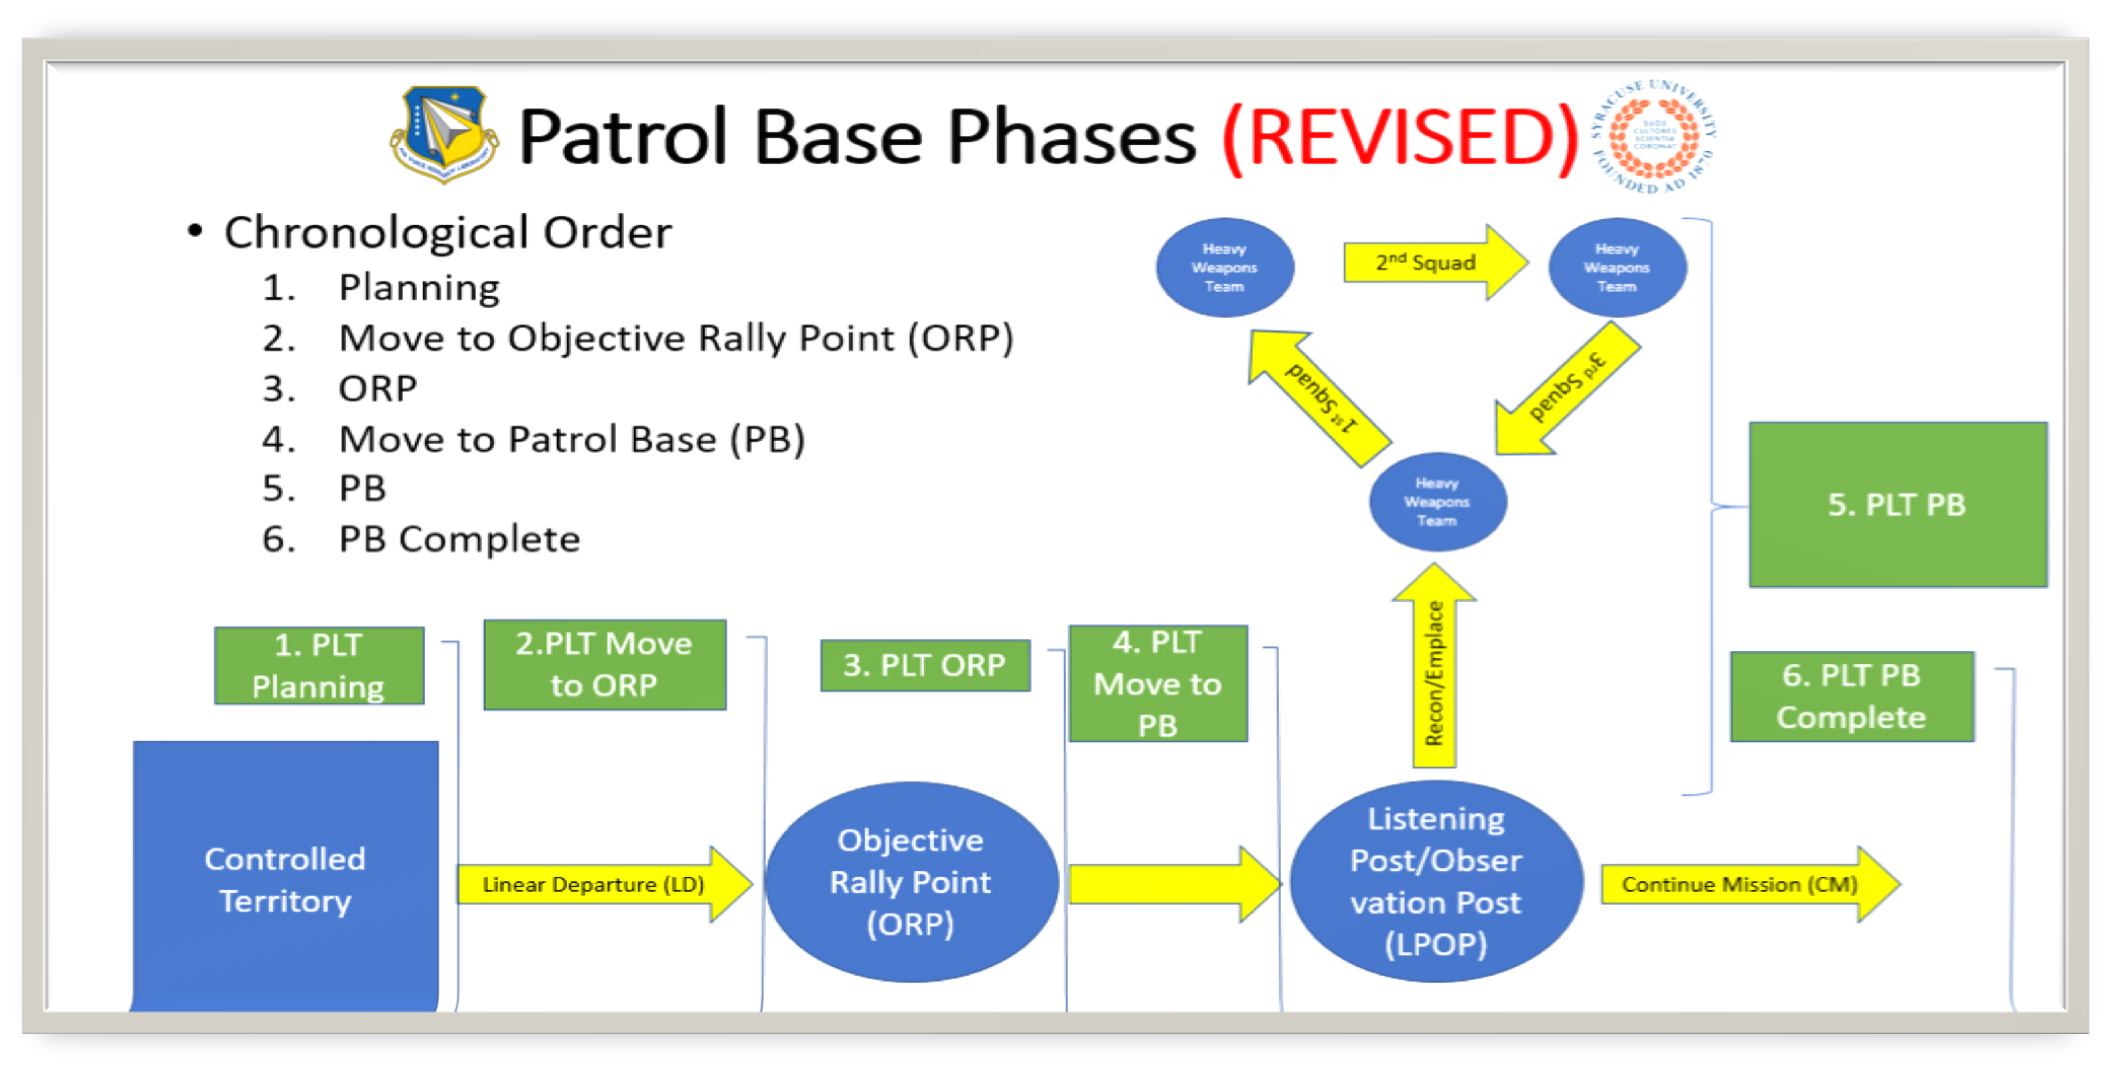
\includegraphics[width=\textwidth]{../figures/pbtoplevel}
\caption{\label{pbtoplevel}A diagram of the most abstract level in the hierarchy of secure state machines.}
\end{figure}

The diagram describes a chronological order of abstract states of the patrol base operations.  The operations begin with the planning phase (1).  Next, they move to the objective rally point (\glsentryshort{orp}) (2). Following this, operations at the \glsentryshort{orp} commence (3).  Afterwards, the patrol base operations move to the actual patrol base (4).  From there, operations at the patrol base proceed (5).  Finally, the patrol base operations are complete (6).  


The next level of abstraction in the hierarchy of \glsentryshortpl{ssm} represents a horizontal slice through the patrol base operations.  In the HOL description is described as the sub level.  This slice describes the patrol base operations at a lower level of abstraction.  It expands each of the states in the top level (except for the last state PB Complete).  For example, the planning phase (1) in figure \ref{pbtoplevel} is expanded into an \glsentryshort{ssm} of its own.  This is called ssmPlanPB.  It consists of several states (see section \ref{sssec:ssmPlanPB}) which detail activities conducted during the planning phase of the patrol base operations.  Each state in the top level (except for PB Complete) has it's own \glsentryshort{ssm} (see the next section).

At yet another lower level of abstraction is the sub sub level.  This level expands upon the states in the sub level \glsentryshortpl{ssm} in the same manner that the sub level expands upon the top level \glsentryshort{ssm}.  

A vertical slice through the diagram is also modeled.  This slice models the patrol base operations from the top level down to the most detailed level.  It begins in the top level phase move to \glsentryshort{orp} (2). Within this state and at the sub level, it falls into the secure halt phase (ssmSecureHalt, see section \ref{sssec:ssmSecureHalt}).  From within this state, it proceeds to the recon phase (ssmORPRecon, see section \ref{sssec:ssmORPRecon}.  Next, it enters the move to glsentryshortpl{orp} phase (ssmMoveToORP4L, see section \ref{sssec:ssmMoveToORP4L}.  Finally, it completes this slice at the form RT phase  (ssmformRT, see section \ref{sssec:ssmFormRT}).

An escape level is also modeled.  Actions in the escape level are reachable from any phase of the patrol base operations.  These actions are the unacceptable circumstances that require the patrol base operations to abort.  For example, if the patrol base contacts the enemy in any phase of the operations, then the command \textit{react to combat} is issued.  The patrol base operations are subsequently aborted.  

In total, there are eight levels of the hierarchy of \glsentryshortpl{ssm}.

   %%%%%%%%%%%%%%%%%%% Section Hierarchy of Secure State Machines %%%%%%%%%%
\section{Hierarchy of Secure State Machines}
\begin{figure}[h]
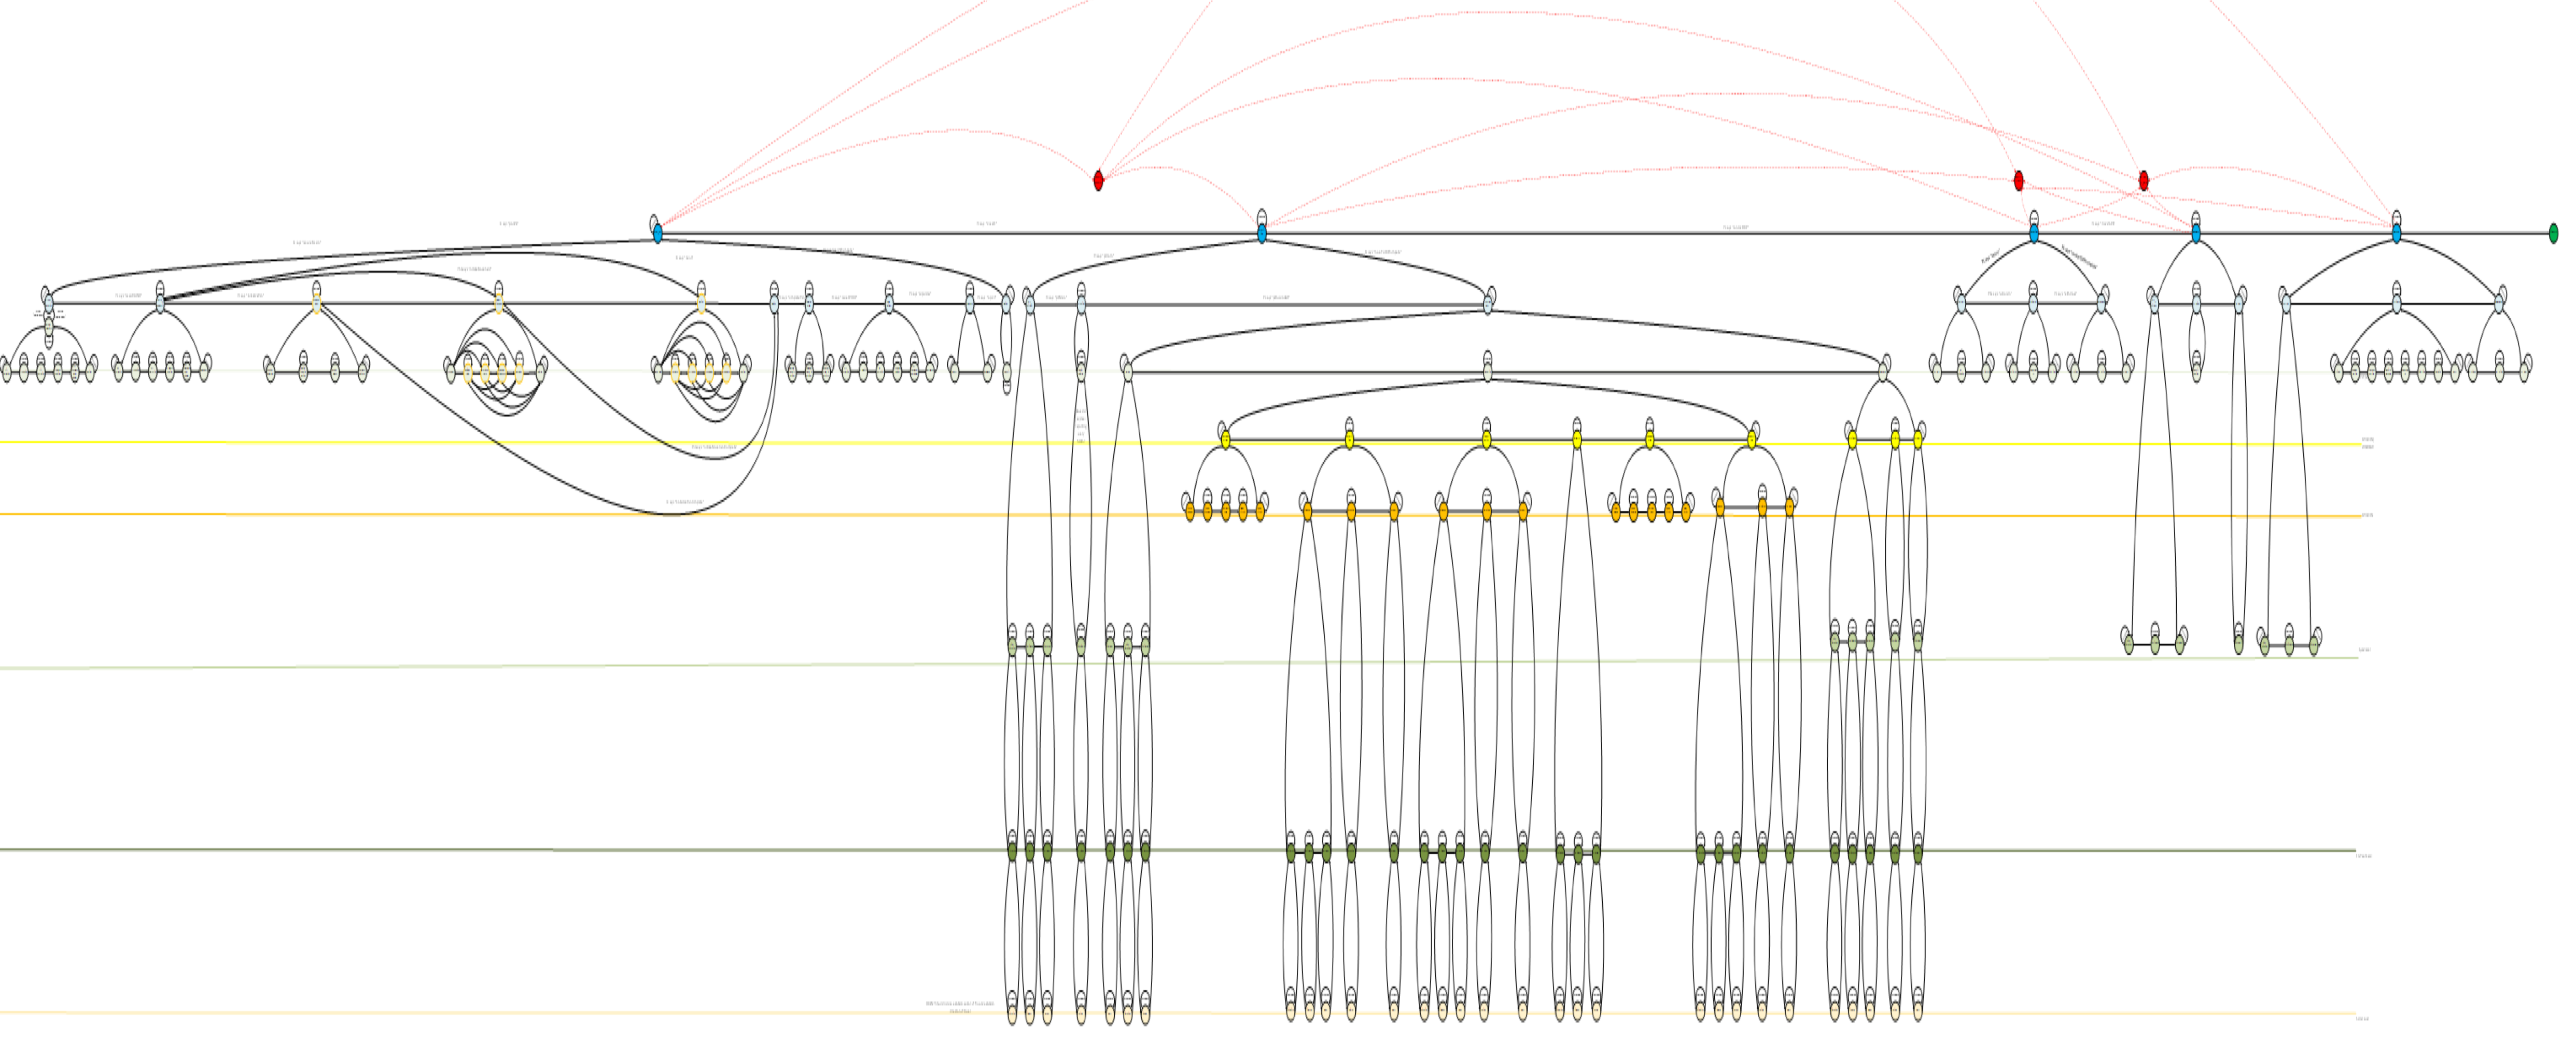
\includegraphics[width=\textwidth]{../figures/overalldiagramsquashed.png}
\caption{\label{overalldiagramsquashed}Diagrammatic description of patrol base operations as a hierarchy of secure state machines.  (Generated by Jesse Nathanial Hall.)}
\end{figure}

          %%%%%%%%%%%%%%%% Subsection Diagrammatic Description %%%%%%%%%%%%%%
\subsection{Diagrammatic Description in Visio}\label{ssec:overalldiagram}
The enormity of the hierarchy of \glsentryshortpl{ssm} is evident in figure \ref{overalldiagramsquashed}.  This is a squashed version of the Visio diagram for the hierarchy of \glsentryshortpl{ssm}.  The diagram is included as a Visio file with the files for this project (LaTeX/figures/diagram.vis).  

The straight, colored lines that span the diagram in figure \ref{overalldiagramsquashed} delineate levels of the hierarchy of \glsentryshortpl{ssm}.  

The small, colored dots in figure \ref{overalldiagramsquashed} represent states (phases) of the patrol base operations.  The labels for these states are not readable in this diagram.  

The states are connected to each other by lines.  These lines represent allowable transitions from one state to another.  The lines are annotated by \glsentryshort{ssm} requests.  For example, a line connecting the top level state PLAN_PB is annotated with the request \textit{PlatoonLeader says crossLD}.  crossLD is an abbreviation for "cross the line of discrimination" and it is the command to transition to the MOVE_TO_ORP state.  If no line connects one state to another then no transition is allowed.

In figure \ref{overalldiagramsquashed}, the red dots at the top of the diagram represent the escape level \glsentryshort{ssm}.  The diagram depicts this \glsentryshort{ssm} as states that are an abstraction above the blue dots (top level states) below.  However, this \glsentryshortpl{ssm} is an exception to the model.  


 

          %%%%%%%%%%%%%%%% Subsection OMNI-Level %%%%%%%%%%%%%%%%%%%%%
\subsection{OMNI-Level}\label{ssec:omnilevel}

          %%%%%%%%%%%%%%%% Subsection Escape %%%%%%%%%%%%%%%%%%%%%%%
\subsection{Escape}\label{ssec:escape}

          %%%%%%%%%%%%%%%% Subsection Top Level %%%%%%%%%%%%%%%%%%%%%%
\subsection{Top Level}\label{ssec:toplevel}

          %%%%%%%%%%%%%%%% Subsection Horizontal Slice %%%%%%%%%%%%%%%%%%%
\subsection{Horizontal Slice}\label{ssec:horizontalslice}

                  %%%%%%%%%%%%% Subsection ssmPlanPB %%%%%%%%%%%%%%%%%%%%%
\subsubsection{ssmPlanPB}\label{sssec:ssmPlanPB}

                  %%%%%%%%%%%%% Subsection ssmMoveToORP %%%%%%%%%%%%%%%%%%%
\subsubsection{ssmMoveToORP}label{sssec:ssmMoveToORP}

                  %%%%%%%%%%%%% Subsection ssmConductORP %%%%%%%%%%%%%%%%%%
\subsubsection{ssmConductORP}label{sssec:ssmConductORP}

                  %%%%%%%%%%%%% Subsection ssmMoveToPB %%%%%%%%%%%%%%%%%%%
\subsubsection{ssmMoveToPB}label{sssec:ssmMoveToPB}

                  %%%%%%%%%%%%% Subsection ssmConductPB %%%%%%%%%%%%%%%%%%%
\subsubsection{ssmConductPB}\label{sssec:ssmConductPB}

          %%%%%%%%%%%%%%%% Subsection Vertical Slice %%%%%%%%%%%%%%%%%%%%
\subsection{Vertical Slice}\label{ssec:verticalslice}

                  %%%%%%%%%%%%% Subsection ssmSecureHalt %%%%%%%%%%%%%%%%%%%
\subsubsection{ssmSecureHalt}\label{sssec:ssmSecureHalt}

                  %%%%%%%%%%%%% Subsection ssmORPRecon %%%%%%%%%%%%%%%%%%%
\subsubsection{ssmORPRecon}\label{sssec:ssmORPRecon}

                  %%%%%%%%%%%%% Subsection ssmMoveToORP4L %%%%%%%%%%%%%%%%%
\subsubsection{ssmMoveToORP4L}\label{sssec:ssmMoveToORP4L}

                  %%%%%%%%%%%%% Subsection ssmFormRT %%%%%%%%%%%%%%%%%%%%
\subsubsection{ssmFormRT}\label{sssec:ssmFormRT}


\end{document}

\glsentryfull{ssm}--glesentryfull

\glsentryfullpl{ssm}--glesentryfullpl


\glsentrytext{ssm}--glsentrytext

\glsentryshortpl{ssm}--glsentryshortpl